\documentclass{article}
\usepackage[utf8]{inputenc}
\usepackage{graphicx}

\title{Instalasi}
\author{itsmeakil707 }
\date{October 2019}
\begin{document}
\title{Instalasi}
\author{Akil Munawwar \\ D4 TI 2B \\ 1184041}
\maketitle

\part{Instalasi}
\section{Instalasi Python}
\begin{enumerate}
    \item Pertama kunjungi https://www.python.org/downloads/release/python-374/
    \item Selanjutnya download file tersebut
    \item Jika sudah, klik dua kali untuk melakukan install
    \item Nanti akan tampil tampilan seperti ini
\end{enumerate}
\begin{figure}[!htbp]
	\centering
		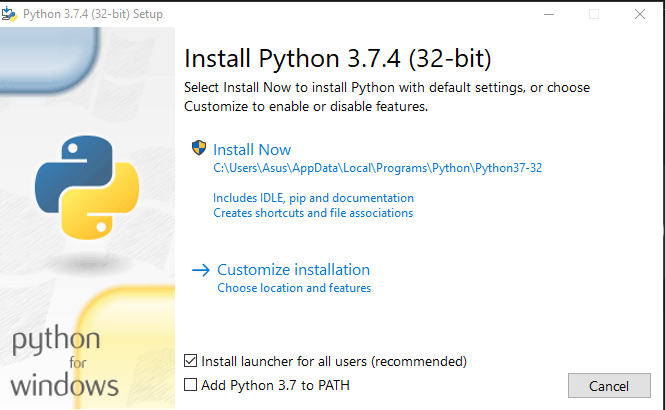
\includegraphics[scale=0.4]{Langkah1.png}
	\caption{Langkah Pertama}
\end{figure}

\newpage
\section{Instalasi PIP}
\begin{enumerate}
    \item Pertama kunjungi https://www.liquidweb.com/kb/install-pip-windows/
    \item Jika sudah, maka cari tulisan \textit{get-pip.py}
    \item Klik kanan dan save file nya ke folder installan python
    \item Jika sudah maka ke cmd dan masuk ke direktori python
    \item Ketik \textit{python get-pip.py}
    \item Tunggu installan hingga selesai
\end{enumerate}
\begin{figure}[!htbp]
	\centering
	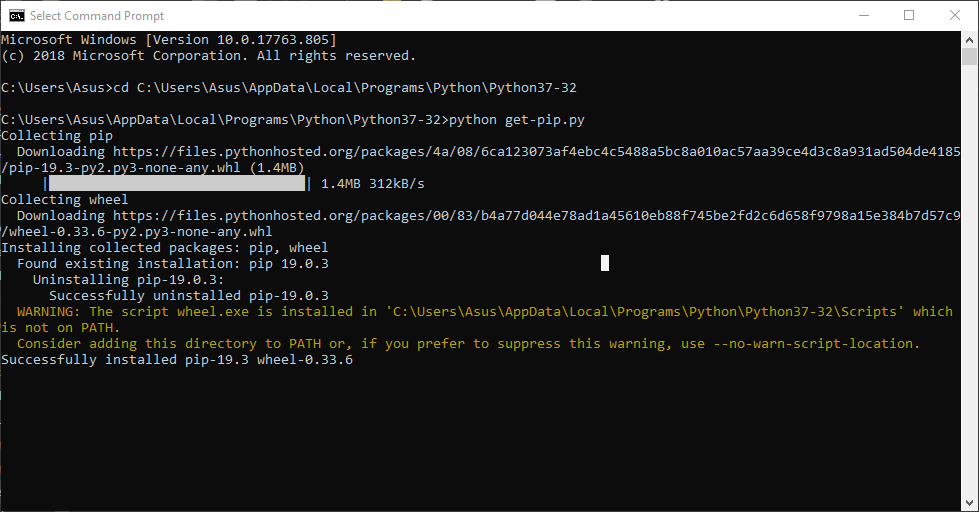
\includegraphics[scale=0.4]{Pip2.PNG}
	\caption{Tunggu hingga selesai}
\end{figure}

\section{Percobaan Enterpreter melalui CMD}
\begin{enumerate}
    \item Pertama buka cmd
    \item Ketik python
    \item Jika sudah masuk ke python nya, maka kita tinggal mencoba untuk membuat perintah hello world
    \item Ketik \textbf{print('hello world')} pada cmd tersebut
    \item Jika sudah maka akan muncul hasil 'hello world
\end{enumerate}
\begin{figure}[!htbp]
    \centering
    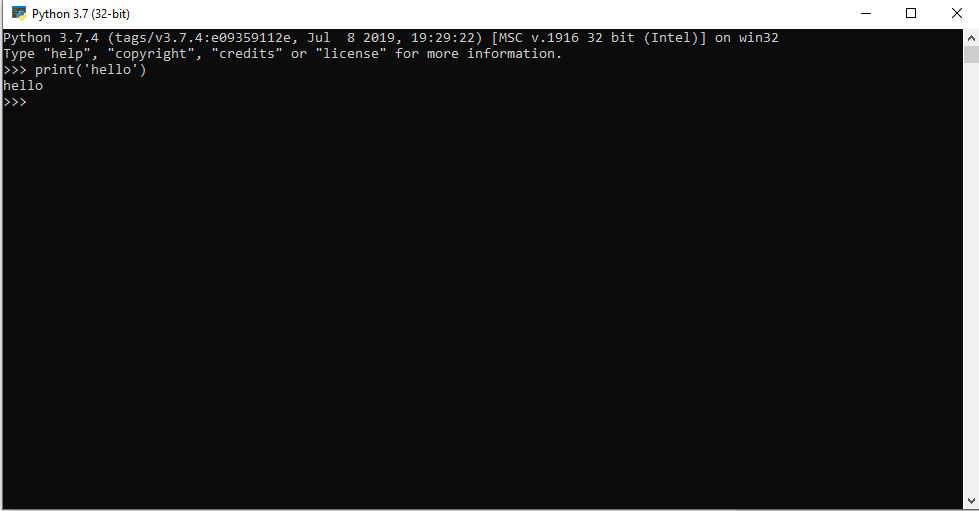
\includegraphics[scale=0.4]{Enterpreter.PNG}
    \caption{Percobaan}
\end{figure}


\newpage
\section{Menjalankan dan Mengupdate Anaconda dan Spyder}
\begin{enumerate}
    \item Pastikan anda sudah menginstall Spyder
    \item Buka Spyder, dan anda sudah berada di Spyder
\end{enumerate}
\begin{figure}[!htbp]
    \centering
    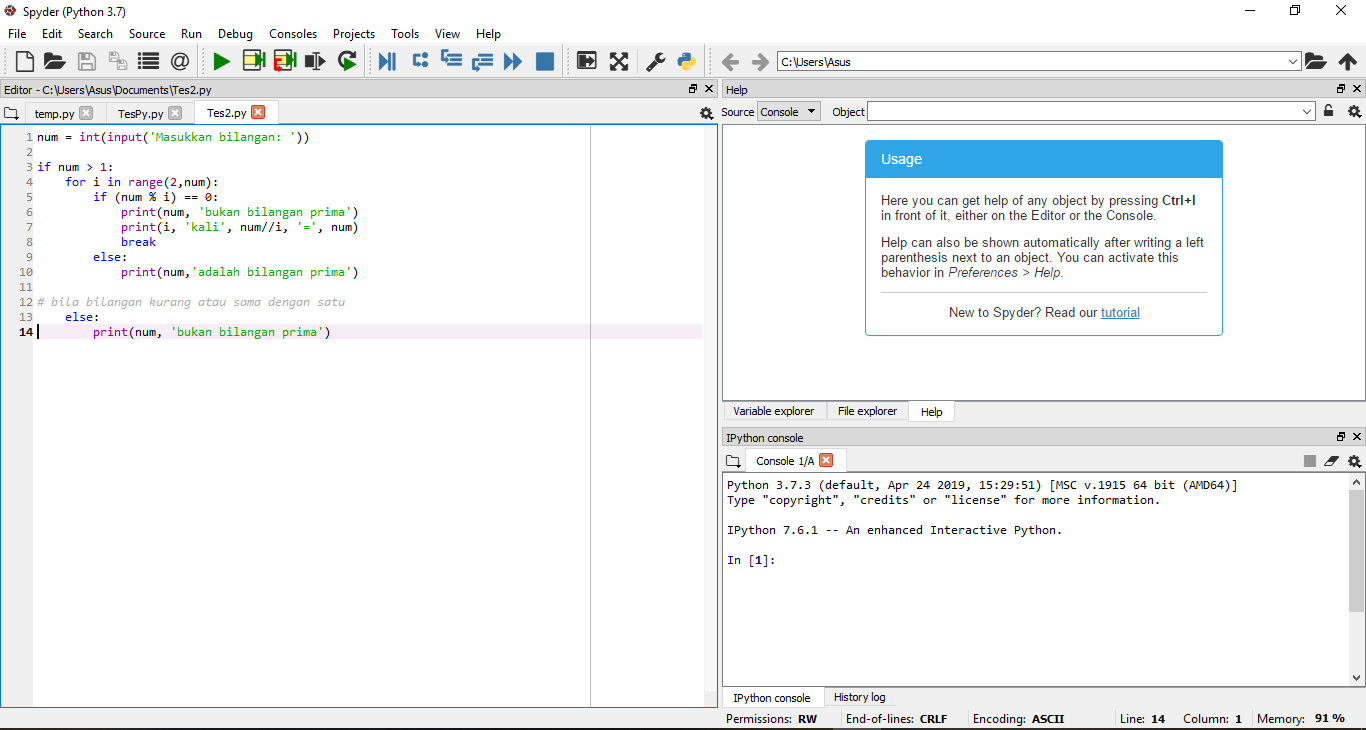
\includegraphics[scale=0.3]{MenjalankanSpyder.PNG}
    \caption{Spyder sudah jalan}
\end{figure}

\newpage
\section{Menjalankan Perintah Hello World di Spyder}
\begin{enumerate}
    \item Pertama, ketikkan perintah print. Perintah ini untuk mencetak output
    \item Kedua, ketikkan kata 'Hello World'. Dibarengin dengan buka dan tutup kurung
    \item Jika sudah maka save dan run
    \item Hasilnya akan terlihat seperti digambar
\begin{figure}
    \centering
    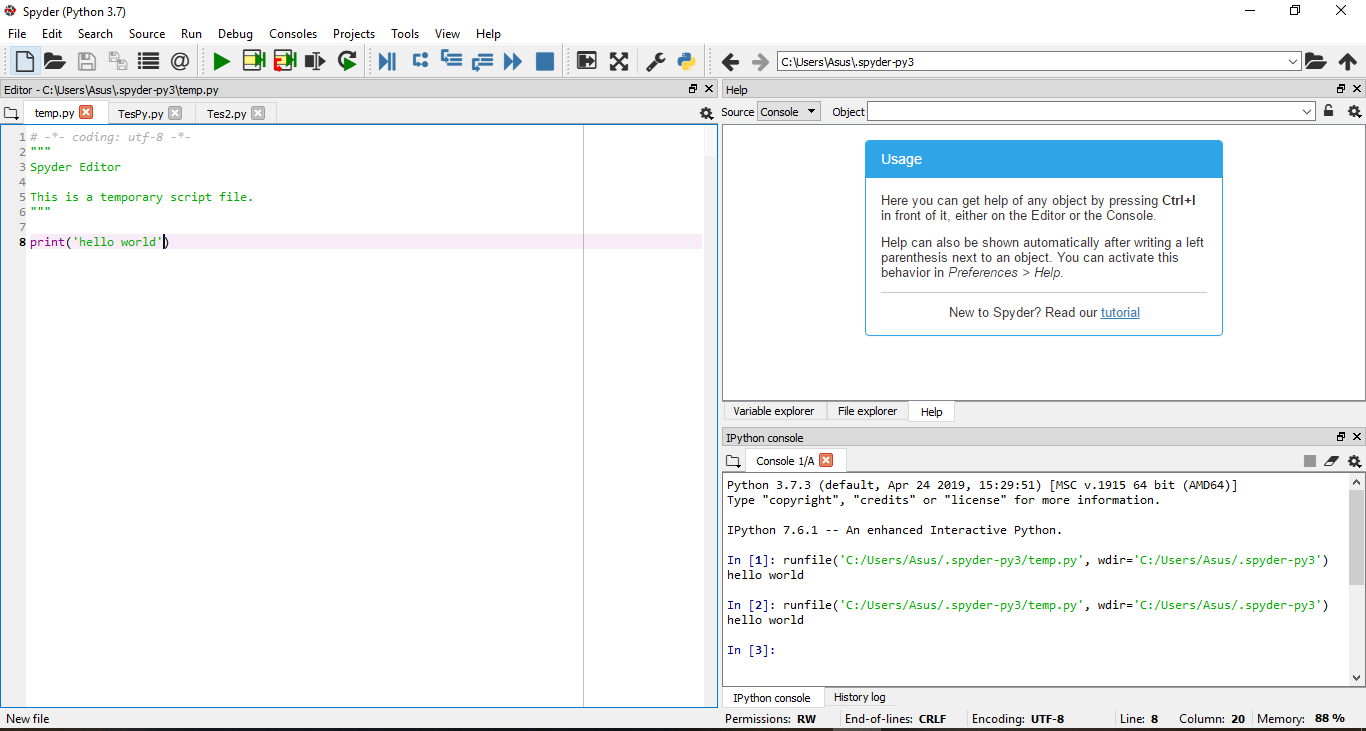
\includegraphics[scale=0.3]{HelloWorld.PNG}
    \caption{Perintah Berhasil}
\end{figure}
\end{enumerate}

\newpage
\section{Auto Login Siap}
\begin{enumerate}
    \item Pertama, buka aplikasi spyder anda
    \item Ketikkan Kodingan seperti ini
\begin{figure}
    \centering
    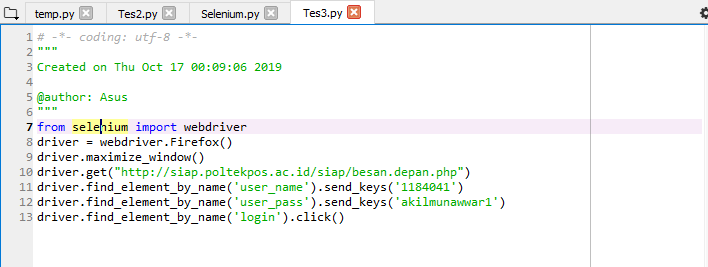
\includegraphics[scale=0.5]{AutoLogin.PNG}
    \caption{Kodingan}
\end{figure}
    \item Setelah itu run, dan auto login telah selesai
\end{enumerate}

\newpage
\section{Variable Explorer}
\begin{enumerate}
    \item Pertama, buat kodingan sesuai selera kalian
    \item Kedua, jika sudah selesai dibuat, maka run
    \item Diatas konsol ada kotak yang berisi variable explorer, file explorer dan help
    \item Klik variable explorer
    \item Disana terdapat tipe data dari kodingan yang kita buat
\begin{figure}
    \centering
    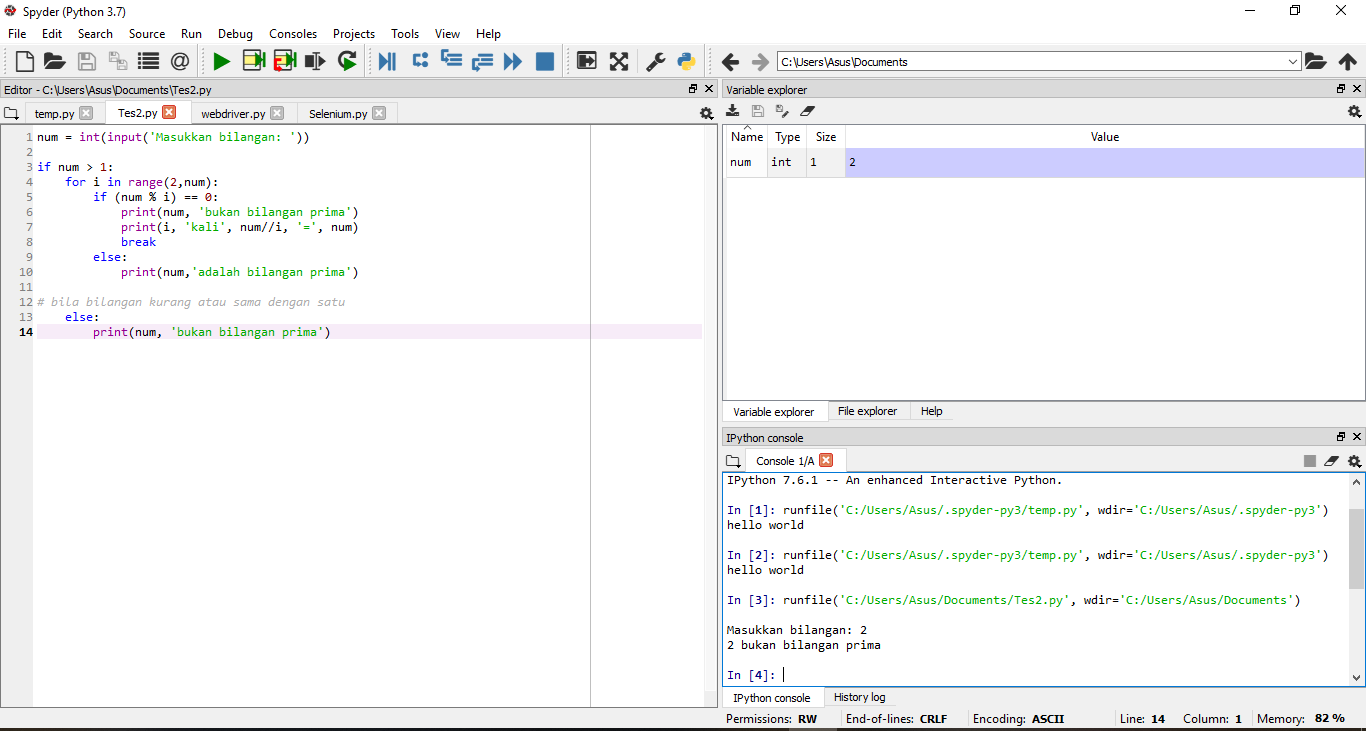
\includegraphics[scale=0.3]{Variable.PNG}
    \caption{Variable Explorer}
\end{figure}
\end{enumerate}
link yt = https://www.youtube.com/channel/UC4fxmBR2GGOsNlnxqsUoukA
\end{document}
